\documentclass[12pt]{report}

\usepackage[margin=1.4in]{geometry}
\usepackage{graphicx}

\usepackage[T1]{fontenc}

\usepackage[francais]{babel}

\usepackage{fontspec}
\setmainfont{Droid Serif}
\setmonofont{Inconsolata}

\usepackage{url}
\usepackage{hyperref}
\usepackage{fancyhdr}
\pagestyle{fancy}

\usepackage{minted}

\linespread{1.3}

\definecolor{gray}{RGB}{155,155,155}
\definecolor{toogyblue}{RGB}{87,102,181}

\usepackage{indentfirst}

\newminted{ocaml} {
  bgcolor=gray!25,
  fontsize=\normalsize,
  mathescape,
  linenos,
  frame=lines,
  framerule=0.3pt
}

\usepackage{titlesec, blindtext}
\definecolor{gray75}{gray}{0.75}
\newcommand{\hsp}{\hspace{20pt}}
\titleformat{\chapter}[hang]{\Huge\bfseries}{\thechapter\hsp\textcolor{gray75}{|}\hsp}{0pt}{\Huge\bfseries}

\fancyhf{}
\rhead{\textbf{\thepage}}
\lhead{\leftmark}
\rfoot{\leftmark}
\lfoot{\textbf{\thepage}}
\renewcommand{\headrulewidth}{0.4pt}
\renewcommand{\footrulewidth}{0.4pt}

\setcounter{tocdepth}{1}


\title{
}

\author{
    Mathieu `RustyCrowbar' Corre \\
    Thibaud `zehir' Michaud \\
    Valentin `toogy' Iovene \\
    Pierre `Grimpow' Gorjux
}

\date{08 décembre 2013}

\begin{document}

\maketitle

\tableofcontents

\chapter*{Introduction}

This document will present the current state of our project, KiBiOCR, as part of
EPITA's syllabus. KiBiOCR's name speaks for itself. It is an OCR (Optical
Character Recognition) program. Its goal is then to recognize characters in a
given image.\\

You will see that our project is breaked up in 5 very distinct parts:

\begin{itemize}
    \item{Lenna}: preprocessing part of the program. Lenna modifies user's input
        image to help other parts of the program to do their job.
    \item{Freddy}: `he' is in charge of the segmentation part, which is
        identifying images, paragraphs, words and characters positions.
    \item{Anna}: this is our artificial neural network (ANN). `She' identifies
        characters segmented by Freddy.
    \item{\emph{(Le petit)} Robert}: this is our dictionary. `He' detects the
        document language and errors made by Anna/Freddy in the identification
        process and then try to find the nearest words.
    \item{Guy}: our user interface. This is the way our program and the user
        will be able to interact.
\end{itemize}

We gave surnames to the parts of our program because we like private jokes but
mainly because shortnames are really convenient when we talk about our project.

% \chapter{The team}
% 
% \section{Valentin `toogy' Iovene}
% 
% \begin{wrapfigure}{l}{0.1\textwidth}
%     \vspace{-1cm}
%     \begin{center}
%         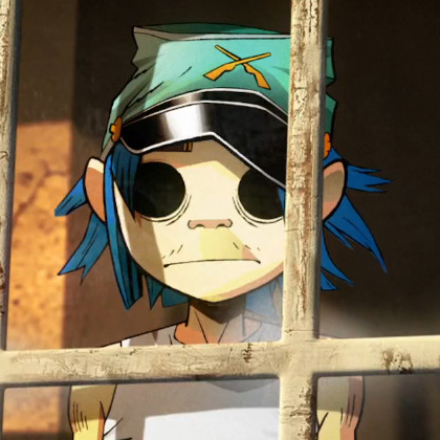
\includegraphics[width=0.1\textwidth]{images/toogy.png}
%     \end{center}
%     \vspace{-1cm}
% \end{wrapfigure}

\chapter{Lenna -- \emph{Preprocessing}}

Before trying to detect paragraphs, lines and characters in the image, and then recognizing the characters, we have to "clean" the image. In this chapter we will describe the different algorithm we implemented in this purpose.

\section{Binarization}
This is the first algorithm we wrote, because it was easy, essential and a good
start to learn the library's basic functions. We first implemented the most
naive algorithm you could think of: computing each pixel's luminosity by
averaging its RGB components, and applying a thresholding. Every pixel below 127
was considered white and every pixel above 128 was considered black.
Of course this was not the definitive algorithm.\\

We could have enhanced it by setting the threshold to the average luminosity,
but it wouldn't have been much better. We instead looked for a better algorithm
and found the Otsu's method to be fitting exactly our purposes. Moreover it is
pretty straightforward to implement. Basically Otsu's method is just a way of
finding the ideal threshold. The ideal threshold is defined as being the one
which minimize the variance between the two classes formed by that threshold.
Therefore it has to try every possible threshold and compute every time the
variance of each class. Thanksfully a little mathematical trick allows us to
significantly reduce the time complexity by maximizing the between-class
variance instead of minimizing the within-class variance.\\

\section{Noise reduction}

We tried two method to reduce the noise in the image: gaussian blur and median
filter. We were unsatisfied with both because letters were less readable after
the filter, and they hardly reduced the noise. We will have to search better
method for noise reduction, but for now we will simply use an algorithm that
removes every black pixel surounded by four white pixels. Even if this is a much
simpler algorithm, letter shapes are saved and some noise is removed.

\section{Rotation}

It is very difficult to detect text zones in the image if they are not straight.
Therefore we will try to detect the angle of the image, and then
rotate it.\\

The first step before rotating the image is to compute the size of the new
image. As for the rest of the algorithm we use rotation matrix, but only on the
corners. From the minimum and maximum horizontally and vertically, we can deduce
the width and height of the rotated image.\\

A naive implementation starts by going through the original image, and
transposing every pixel $(x, y)$ into the corresponding one in the rotated
image. We do that by computing the dot product between the pixel's coordinates
and the rotation matrix of the given angle. We want to turn the image with the
center of the image as the origin, so we have to add half of the width
(respectively height) of the image to $x$ (respectively $y$) before actually
computing the rotated point. It turns out to be a pretty bad algorithm, because
not every pixel of the rotated image will have an antecedent in the original
image. This is due to the fact that some pixels in the original image have the
same corresponding rotated pixel, because of the rounding made to get integer
coordinates. This creates an aliasing effect.\\

Instead, we need to make the reverse operation: take every pixel from the new
empty image, and find its corresponding pixel in the original image. Therefore,
the only thing to do is to apply a rotation matrix with the opposite angle.\\

Because of the imprecision of the integer coordinates, the rotated image is
still not perfect. A potential improvement will be to use an algorithm that
takes this imprecision into account, like the bilinear interpolation.

\subsection{Angle detection}
\subsubsection{Hough transform}

The Hough transform is a general method for finding lines and ellipses in an
image. It is often used because once the mathematical principle is understood,
it is not that hard to implement, and it has a much lower time complexity and
better results than some other methods like Fourier transform. For our purposes,
we only need to handle the most simple case: line detection in a binary image.\\

The Hough transform relies on a very particular representation of lines of the
plane: instead of being as the two parameters $a$ and $b$ in the classical
equation $y = ax + b$, it is described as the couple $(r, \theta)$ where $r$ is
the distance of the line from the origin and $\theta$ is the angle of this
distance from the absciss.\\

\begin{center}
\end{center}

How is this representation useful ? It comes from the fact that, given a point
of coordinates $(x, y)$ and the angle $\theta$ of a line going through this
point, we can express very simply the distance $r$ of the line from the origin.
The equation is as follows:\\

$r = x\cos\theta + y\sin\theta$\\

So for a point of coordinates $(x, y)$ we can plot the graph of $r$ in function
of $\theta$. It is easy to guess from the equation that it will be a sinusoid.
This sinusoid represents the set of lines going through this particular point.
Now if we store this graph on an accumulator, and add to this accumulator the
sinusoid of every other points, here is what happens:\\

\begin{center}
\end{center}

Clearly there is a point where all sinusoids cross. The coordinates of this
point represents the values $r$ and $\theta$ of the line going through every
point at once.

\subsubsection{More preprocessing}

There is still one thing to fix before applying the Hough transform to our
scanned image: A text doesn't appears as a straight line. We tried to apply the
Hough transform directly to a binarized document, but most of the time it would
find either the diagonal of the document (since the diagonal goes through more
black points than an horizontal or a vertical line), or the angle of a prominent
bookbinding or document border. After a few researches, we came with our own
solution: we first find "blocks" of pixels, defined as being a set of conjoint
pixels. We remove every pixel of this block and replace them by a single pixel
at the center of the block. There are two purposes to this algorithm: replacing
every character by its center to make text lines apparent, and reducing the
importance of large blocks of pixels as bookbindings and images in the Hough
transform. Here is a sample output:\\

\begin{figure}[h!]\
    \centering
    \caption{input image}
\end{figure}
\begin{figure}[h!]\
    \centering
    \caption{center of each block}
\end{figure}
\begin{figure}[h!]\
    \centering
    \caption{line found by the Hough transform}
\end{figure}

This method has a major flaw that we wish to correct before the end of the
project: when the noise isn't reduced enough, every separate pixel in the
"noisy zone" is considered a block and gets a huge role in the Hough transform,
potentially leading the angle detection to fail completely. Every further step
of the OCR relies on a perfectly straight image, and it is therefore very
important that we correct this. \\

\section{TODO}

If Lenna is almost finished, some improvements still remain:

\begin{itemize}

    \item{Rotation}: it is divided in two parts: angle detection, which is done
        and the real rotation. The current algorithm gives very poor results. We
        are going to implement bicubic interpolation which is a standard in many
        image editing programs (including Adobe Photoshop).
    
    \item{Noise reduction improvement}: our noise reduction algorithm is not
        strong enough on some images. Sometimes it fails and Freddy cannot work
        with Lenna's output.

    \item{Hough transform preprocess} The method we use has a major flaw that we wish to correct before the end of
        the project: when the noise isn't reduced enough, every separate pixel
        in the "noisy zone" is considered a block and gets a huge role in the
        Hough transform, potentially leading the angle detection to fail
        completely. Every further step of the OCR relies on a perfectly straight
        image, and it is therefore very important that we correct this.

    \item{Image scaling}: Guy may need an image scaling algorithm to display
        thumbnails of user's image.

\end{itemize}

\chapter{Freddy -- \emph{Segmentation}}

Freddy is our segmentation module. It uses OCSFML.
To detect lines as today, we first assume that all the previous preprocessing steps were done perfectly, which means no artefacts, good rotation, binarization... For now, we can only get text, in one column, and no images. We will work on those situations, and Freddy will be working as expected on time.

\begin{center}
\end{center}

\begin{center}
\end{center}

\section{Line and character detection}

\subsection{Making horizontal/vertical histogram}

To detect lines, we need to make histograms, containing the number of black pixels in every line/column of line of pixel of the provided image.We put everything in lists.

\subsection{Delimit lines/characters}

When the number of black pixel changes a lot, we decide to create or to end a line/to create or end a character. We put it in lists

\chapter{Anna -- \emph{Identification}}

After we have preprocessed the image and found the paragraphs, lines and characters in the document, we need to recognize these characters. To do this, we use a machine learning technique called a feed-forward neural network. In this chapter, we will describe in detail the result of our researches on the subject.

\section{Machine learning}

Machine learning is a field of research in which we try to design "agents" able
to improve their performance on a given task with experience. In the case of an
OCR software, the agent's task will be to classify images of characters, and the
experience will consist of feeding the agent with many examples. The examples
will be pairs of the form (image of the character, corresponding character).

\section{Univariate linear regression}

Lets look at a simpler problem: we have examples of the form $(x, y)$ where $x$
and $y$ are numbers, and our goal is to find a straight line to fit the
examples.\\

\begin{center}
\end{center}

The line will be of the form $h_w(x) = w_1x + w_0$. In order to determine the
most fitting line, we first need to define an error function. The sum of the
squared error appears to have nice properties (as being positive and
differentiable). This error function is expressed as follows:
$Loss(h_w) = \sum\limits_{j=1}^{N}(y_j - h_w(x_j))^{2}$. Now we need to minimize
this. To understand how we do this, it helps to visualize the graph ofthe Loss
in function of $w$.\\

Now imagine we start at a random point on this graph (i.e., we start with a
random line). To get to the minimum of the function, we only need to follow the
slope downward. Mathematically, this translates as substracting the gradient of
the Loss function from the current point, since the gradient points toward the
steepest slope upward. We usually multiply the gradient by a constant called the
learning rate, noted $\alpha$, to regulate the size of the steps. A slow
learning rate means converging slowly but a large learning rate might lead to
stepping over the minimum. The update rule is then:\\

$w_i \leftarrow w_i - \alpha \frac{\partial}{\partial w_i} Loss(w)$\\

We won't compute the derivative right now as we don't need it.

\section{Multivariate linear regression}

The extension to a multivariate problem is pretty straight forward. Lets denote
by $\textbf{x} = (x_0, x_1, ..., x_n)$ the input vector. The estimation function
then becomes $h_w(\textbf{x}) = w_nx_n + ... + w_1x_1 + w_0x_0$.

\section{Logistic regression}

What we want is a classification algorithm. We only need to slightly modify the
previous algorithm to make it a binary classifier: we keep the estimation
function $h_w(x)$, but we then feed the result to another function whose output
is in $[0;1]$. One such function is the step function, which worth 0 if $h_w(x)$
is negative and 1 otherwise. But this function is not differentiable, and we
will see later that it is a problem. So we usually prefer the logistic function,
or sigmoid function:\\

\begin{center}
\end{center}

Its equation is $g(x) = \frac{1}{1 + e^{-x}}$, and its derivative is
$g(x)(1 - g(x))$. Applying the same algorithm as for the multivariate linear
regression, the update rule becomes:\\

$w_i \leftarrow w_i + \alpha (y - h_w(\textbf{x}))
h_w(\textbf{x})(1 - h_w(\textbf{x}))x_i$\\

There is no need here to explain the derivation of the Loss function.

\section{Perceptron}

The logistic regression function will be the elementary brick for our neural
network. It is what we will call a neuron, since it is very close to the real
principle of biological neuron. Now lets complexify the problem a little bit: we
need to classify the input data between more than two possible outcomes. Let's
say for example that we need three possible outcomes. We only need to connect
the input to three different logistic regression units. This will produce an
output vector instead of a single value, and ideally this vector will converge
toward something like (1, 0, 0), (0, 1, 0) or (0, 0, 1), each time representing
one of the three possible cassifications. This is called a single-layer
feed-forward neural network, or perceptron.\\

\begin{center}
\end{center}

\section{multi-layer feed-forward neural network}

A feed-forward neural network is a perceptron, whose output will be the input of
another perceptron, etc. until it reaches the output layer. Every layer that is
not the input layer or the output layer is called a hidden layer. The big
advantage of a multi-layer feed-forward neural network over a perceptron is that
it can potentially compute any continuous function with only one hidden layer
and with the right number of neurons in each layer, according to the universal
approximation theorem.\\

\begin{center}
\end{center}

What changes between the perceptron and the multi-layer feed-forward neural
network is the derivative of the loss function. Once again, there is no need to
enter into the details of the maths behind the derivation, but the only thing we
need to know when implementing the neural network is that the derivative of the
parameters in one layer depends on the derivative of the parameters of the next
layer. Therefore we need to compute the derivative in the output layer, then the
hidden layer, hence the term "backpropagation".

\section{Optimizations}

The only optimization we implemented at this point is the momentum. In the
gradient descent process, we can consider that the current point has some
inertia by adding a certain percentage of the gradient of the last iteration in
the update rule. There are two purposes to this: converging faster, and avoiding
local minimum.

\chapter{Robert -- \emph{Spell checking}}

Robert is a module, which can detect the language used in a given text, and eventually indicate
to the user which word is wrong, and give a selection of possible corrections.

\section{Generation of Dictionnaries}
A dictionnary is a file which contains a lot of words of a specific language we can find in
a text.\\
We didn't create them ; it's too long and we can easily find some complete dictionnaries on
Internet (~150 000 words in English, ~700 000 words in French, for example).\\
But actually, searching a word in a file is'nt a really good idea and may take a long time.
That's why before doing anything else, we have to generate a data structure which will store
the whole words of the dictionnary file. This one is a hashtable, because the
time taken to search a common word is constant.\\
So, when loading Robert, OCaml will generate the whole dictionnaries needed by creating hashtables
and put them in a list.\\
\\
But there is still a problem : the time taked to create a hashtable from a dictionnary is around 1
second. If we want to accept many differents languages, the loading of the module would be too long.
The solution is the Marshall module : it let us serialize an object into a bytes array, and save it
into files. The opposite procedure is also possible.
So OCaml has juste to read the byte array and deserialize it to load a hashtable. This technic need
more memory but is really faster (around 1000\% faster)
\section{Detecting language in a given Text}
The algorithm used is pretty simple: it will analyse the first X words (X is an empirical number, set
as 200). 
For each language, it will count the number of words recognised ; The final language is the one which has the mosts of right matches.
\section{Detection of wrong words}
It's quite the same thing. The algorithm make a list, and starts to read the whole text. Each time a word is wrong, it is added to the list.
\section{Selection of possible corrections for a wrong word}
Generally, when a word is wrong, it's because the user writted it thinking about a right word, with the same pronunciation.\\
That's why the Soundex algorithm has been used in our project. It transforms a given string into its phonetic equivalent.
So, we created a new type of dictionnary : a "phonetic hashtable" : we can find the word by searching the phonetic string.
So, if we're searching a phonetic string we can find the whole words which have the same phonetic string.
We have a first list with a lot of possible corrections.\\
But we won't give for examples 42 possibilies of correction to a wrong word: the user would be lost ; that's why we'll give
to the user only 5 possibilities.\\
The possibilities will be sorted using another algorithm, called Levenshtein.
Levenshtein calculates the number of modifications we have to make in order to change a word A into a word B.
So, we'll only have the 5 words which are the closest to the wrong word. 
 
\chapter{Guy -- \emph{Graphical User Interface}}

\section{A quick overview of Guy}

Guy is our GUI. It uses LablGTK and OCSFML, and will probably be using html to render the text output. It has several roles that we will describe right now. It is today composed of one window, to choose the file. It will be, for the second soutenance, composed of two or three more windows, to show the flow of the processing and the time taken by every main algorithm that we are using. 

\begin{center}
\end{center}

\section{A user-friendly interface}

\subsection{Helping the user to choose the image to process}

Guy has a built-in file browser, which is very intuitive, and easy to use, to select the file you want to use. Once the file has been selected, it's path will be displayed in an editable text box. However, the user can directly type in the provided text box the path of his desired file. Of course, it is still possible to use our program via the command-lines.

\subsection{Displaying the usefull informations}

We will display a miniature image of the image (assuming that it really is an image) that the user choosed.

\subsection{Showing the final result to the user}

Guy will be charged to show to the user the final work of our OCR. Indeed, we will present the image the user gave us, and the text we could detect, with the eventual orthograph corrections using Robert. It needs to be well organised, so that in case of a long document, the user could find where everything in the output text is located in his image, and vice-versa.

\section{Guy is the foreman}

One of the role of our GUI is to make every module work one after the other, calling them one after the other, with the right parameters. It will be possible to include one or several progress bars to inform the user of the flow of the processing.

\chapter{Website}

\section{Python}

\begin{center}
\end{center}

This year, we decided to switch from PHP to Python. We think that Python is a
stronger and more relevant language and we wanted to learn its syntax and its
specifics. So, here we are. \\

Plus, if we want to put our OCR online so that people can use it via a web
interface, it would me so much easier to do it with Python than with PHP. Python
can easily call other programs and execute commands on the server in a very
secure way. It is more complicated with PHP.

\section{Django}

\begin{center}
\end{center}

There is a very nice Python web framework out there on the web that is called
Django. Working with Django is quick: it is made for rapid development and for
perfectionists (we are).

\section{Nginx}

\begin{center}
\end{center}

We wanted to use something else than a basic Apache server so we decided to go
with Nginx, a quick, clean and easy to configure web server.

\section{Github}

\begin{center}
\end{center}

Our code is hosted on the now very famous website (and git server) GitHub. For
the moment, it is located in a private repository (for obvious reasons) but we
plan to go opensource once the last soutenance will be passed!

\chapter*{Conclusion}

Our project is moving forward very well. Our team is organized, we are all
working with passion and seriousness. We often schedule meetings and establish
task lists so that everyone is aware of what has to be done and can pick up
something he is interested in. \\

Some very tough tasks are waiting for us and we hope we will be able to show up
at the final with a fresh and working piece of art.

\end{document}


